\documentclass[aspectratio=169, 14pt]{beamer}
\usepackage[utf8]{inputenc}
\usepackage[english]{babel}
\usepackage{tipa}
\usepackage{graphicx}
\usepackage{transparent}
\usepackage[ruled, lined, linesnumbered, commentsnumbered]{algorithm2e}
\usepackage{pgfplots}
\newcommand\mycommfont[1]{\small\ttfamily\textcolor{blue}{#1}}
\SetCommentSty{mycommfont}
\renewcommand{\thealgocf}{}
\usepackage{setspace}
\usepackage{tikz}
\usetikzlibrary{matrix,backgrounds}
\usetikzlibrary{arrows}
\usetikzlibrary {arrows.meta}
\usetikzlibrary{calc,shadows.blur,fit,positioning}
\usetikzlibrary{shapes.multipart,chains}
\usepackage{minted}
\usepackage{fontawesome5}
\usepackage{booktabs}
\usepackage{caption}
\usepackage{hyperref}
\hypersetup{
    colorlinks=true,
    linkcolor=blue,
    filecolor=magenta,      
    urlcolor=cyan,
    }
\urlstyle{same}
\usetheme{metropolis}
\metroset{block=fill}
\usecolortheme{default}
\definecolor{darkmidnightblue}{rgb}{0.0, 0.2, 0.4}
\definecolor{LightGray}{gray}{0.9}


%------------------------------------------------------------
%This block of code defines the information to appear in the
%Title page
\title[Data Structures] %optional
{Data Structures}

\subtitle{Lab}

\author[CHEN Zhongpu] % (optional)
{CHEN Zhongpu}

\institute[] % (optional)
{
  School of Computing and Artificial Intelligence \\
  \href{mailto:zpchen@swufe.edu.cn}{zpchen@swufe.edu.cn}
}

\date[] % (optional)
{SWUFE, Fall 2022}

%End of title page configuration block
%------------------------------------------------------------


%------------------------------------------------------------
%The next block of commands puts the table of contents at the 
%beginning of each section and highlights the current section:

% \AtBeginSection[]
% {
%   \begin{frame}
%     \frametitle{Table of Contents}
%     \tableofcontents[currentsection]
%   \end{frame}
% }
%------------------------------------------------------------


\begin{document}

%The next statement creates the title page.
\frame{\titlepage}

%---------------------------------------------------------
%This block of code is for the table of contents after
%the title page
% \begin{frame}
% \frametitle{Table of Contents}
% \tableofcontents
% \end{frame}
%--------------------------------------------------------
\begin{frame}
    \frametitle{Review}
    \begin{enumerate}
        \item Stack
        \item Queue (deque)
        \item Linked list
    \end{enumerate}
\end{frame}

{
    % \usebackgroundtemplate{\transparent{0.3}{\begin{picture}
    %     \includegraphics[height=0.7\paperheight]{cover}
    % \end{picture}    
    % }}
\usebackgroundtemplate{
  \tikz[overlay,remember picture] 
  \node[opacity=0.3, at=(current page.south east),anchor=south east, yshift=2cm,xshift=4cm] {
    \includegraphics[height=0.6\paperheight]{cover}};
}
    \begin{frame}
        \section{\textcolor{darkmidnightblue}{1. Lab}}
    \end{frame}

}


\begin{frame}

    \section{\textcolor{darkmidnightblue}{2. Recursion}} 

    \begin{quote}
        Recursion (adjective: recursive) occurs when a thing is defined in terms of itself or of its type.
    \end{quote}

\end{frame}

\begin{frame}[fragile]
    \frametitle{2.1 Example}

\begin{columns}
    \column{.5\textwidth}<1->
    The \textbf{Fibonacci} sequence:
\begin{itemize}
    \item $F(0) = 0$
    \item $F(1) = 1$
    \item $F(2) = 1$
    \item $F(n) = F(n - 1) + F(n - 2)$
\end{itemize}
    \column{.5\textwidth}<2->
    The \textbf{Linked list}:

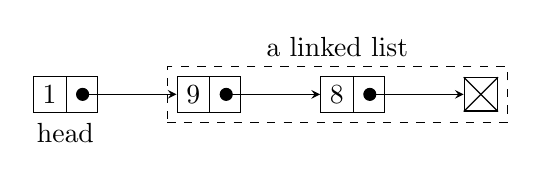
\begin{tikzpicture}[list/.style={rectangle split, rectangle split parts=2,
    draw, rectangle split horizontal}, >=stealth, start chain]

  \node[list,on chain] (A) {1};
  \node[list,on chain] (B) {9};
  \node[list,on chain] (C) {8};
  \node[on chain,draw,inner sep=6pt] (D) {};
  \draw (D.north east) -- (D.south west);
  \draw (D.north west) -- (D.south east);
  \draw[*->] let \p1 = (A.two), \p2 = (A.center) in (\x1,\y2) -- (B);
  \draw[*->] let \p1 = (B.two), \p2 = (B.center) in (\x1,\y2) -- (C);
  \draw[*->] let \p1 = (C.two), \p2 = (C.center) in (\x1,\y2) -- (D);
  \node[below=of A, yshift=1cm] (head){\alert{head}};

  \node[fit=(B)(C)(D), dashed, draw](remain) {};

  \node[above=of remain, yshift=-1cm]{\alert{a linked list}};

\end{tikzpicture}
\end{columns}

\end{frame}

\begin{frame}[fragile]
    \frametitle{2.2 Recursive Algorithm}

    \begin{itemize}
        \item Base step
        \item Recursive step
    \end{itemize}
    
    \begin{minted}[bgcolor=LightGray]{python}
def fibonacci(n):
    if n == 0:
        return 0
    elif n == 1 or n == 2:
        return 1
    else:
        return fibonacci(n - 1) + fibonacci(n - 2)        
    \end{minted}
\end{frame}

\begin{frame}[fragile]
 Get the length of a list recursively:
 \begin{equation*}
    \begin{split}
    length([1, 9, 8]) & = 1 + length([9, 8]) \\
     & = 1 + 1 + length([9]) \\
     & = 1 + 1 + 1 + length([]) \\
     & = 1 + 1 + 1 + 0
    \end{split}
\end{equation*}

    \begin{minted}[bgcolor=LightGray]{python}
def len_of_list(a):
    if len(a) == 0:
        return 0
    return 1 + len_of_list(a[1:])
\end{minted}

\end{frame}

\begin{frame}
    \frametitle{Exercise}
\begin{columns}
    \column{.5\textwidth}
    Given a linked list with \alert{head}, how to get its length recursively?
    \column{.5\textwidth}
    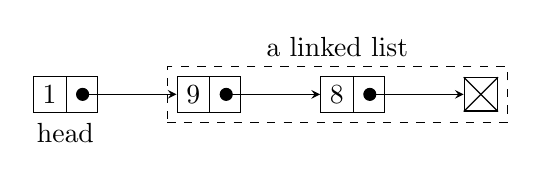
\begin{tikzpicture}[list/.style={rectangle split, rectangle split parts=2,
        draw, rectangle split horizontal}, >=stealth, start chain]
    
      \node[list,on chain] (A) {1};
      \node[list,on chain] (B) {9};
      \node[list,on chain] (C) {8};
      \node[on chain,draw,inner sep=6pt] (D) {};
      \draw (D.north east) -- (D.south west);
      \draw (D.north west) -- (D.south east);
      \draw[*->] let \p1 = (A.two), \p2 = (A.center) in (\x1,\y2) -- (B);
      \draw[*->] let \p1 = (B.two), \p2 = (B.center) in (\x1,\y2) -- (C);
      \draw[*->] let \p1 = (C.two), \p2 = (C.center) in (\x1,\y2) -- (D);
      \node[below=of A, yshift=1cm] (head){\alert{head}};
    
      \node[fit=(B)(C)(D), dashed, draw](remain) {};
    
      \node[above=of remain, yshift=-1cm]{\alert{a linked list}};
    \end{tikzpicture}
    
\end{columns}

\scalebox{.85}{  
        \begin{algorithm}[H]
        \caption{length(head)}
\If{head == null} {
    \Return{0}
}
\Return{1 + length(head.next)}
        \end{algorithm}
}
    
\end{frame}

\begin{frame}
    \frametitle{2.3 Reverse A List}
    
    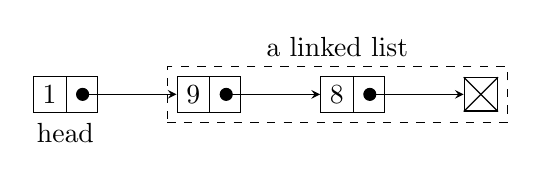
\begin{tikzpicture}[list/.style={rectangle split, rectangle split parts=2,
        draw, rectangle split horizontal}, >=stealth, start chain]
    
      \node[list,on chain] (A) {1};
      \node[list,on chain] (B) {9};
      \node[list,on chain] (C) {8};
      \node[on chain,draw,inner sep=6pt] (D) {};
      \draw (D.north east) -- (D.south west);
      \draw (D.north west) -- (D.south east);
      \draw[*->] let \p1 = (A.two), \p2 = (A.center) in (\x1,\y2) -- (B);
      \draw[*->] let \p1 = (B.two), \p2 = (B.center) in (\x1,\y2) -- (C);
      \draw[*->] let \p1 = (C.two), \p2 = (C.center) in (\x1,\y2) -- (D);
      \node[below=of A, yshift=1cm] (head){\alert{head}};
    
      \node[fit=(B)(C)(D), dashed, draw](remain) {};
    
      \node[above=of remain, yshift=-1cm]{\alert{a linked list}};
    \end{tikzpicture}

    \scalebox{.8}{  
        \begin{algorithm}[H]
            \setstretch{.9}
            \caption{reverseList(head)}
            $pre\gets null$ \\
            $cur\gets head$ \\
            \While{cur $\neq$ null} {
                $next\gets cur.next$ \\
                $cur.next\gets pre$ \\
                $pre\gets cur$ \\
                $cur\gets next$
            }
            \Return{pre}
            \end{algorithm}
    }

\end{frame}

\begin{frame}
\begin{itemize}
    \item \textbf{Case 1}: the list is empty.
    \item \textbf{Case 2}: the size is 1.
    \item \textbf{Case 3}: the size is greater than 1.
\end{itemize}

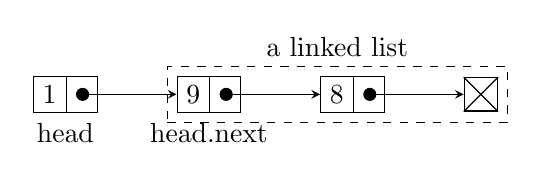
\begin{tikzpicture}[list/.style={rectangle split, rectangle split parts=2,
    draw, rectangle split horizontal}, >=stealth, start chain]

  \node[list,on chain] (A) {1};
  \node[list,on chain] (B) {9};
  \node[list,on chain] (C) {8};
  \node[on chain,draw,inner sep=6pt] (D) {};
  \draw (D.north east) -- (D.south west);
  \draw (D.north west) -- (D.south east);
  \draw[*->] let \p1 = (A.two), \p2 = (A.center) in (\x1,\y2) -- (B);
  \draw[*->] let \p1 = (B.two), \p2 = (B.center) in (\x1,\y2) -- (C);
  \draw[*->] let \p1 = (C.two), \p2 = (C.center) in (\x1,\y2) -- (D);
  \node[below=of A, yshift=1cm] (head){\alert{head}};

  \node[below=of B, yshift=1cm] {\alert{head.next}};

  \node[fit=(B)(C)(D), dashed, draw](remain) {};

  \node[above=of remain, yshift=-1cm]{\alert{a linked list}};
\end{tikzpicture}

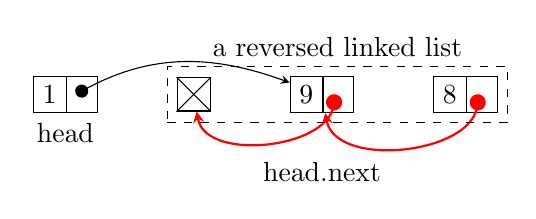
\begin{tikzpicture}[list/.style={rectangle split, rectangle split parts=2,
    draw, rectangle split horizontal}, >=stealth, start chain]

  \node[list,on chain] (A) {1};
  \node[on chain,draw,inner sep=6pt] (D) {};
  \draw (D.north east) -- (D.south west);
  \draw (D.north west) -- (D.south east);
  \node[list,on chain] (B) {9};
  \node[list,on chain] (C) {8};

  \draw[*->, red, thick] let \p1 = (C.two), \p2 = (C.center) in (\x1,\y2) to[out=-80,in=-80] (B);
  \draw[*->, red, thick] let \p1 = (B.two), \p2 = (B.center) in (\x1,\y2) to[out=-80,in=-80] (D);
  \draw[*->] let \p1 = (A.two), \p2 = (A.center) in (\x1,\y2) to[out=30,in=160] (B);
  \node[below=of A, yshift=1cm] (head){\alert{head}};

  \node[below=of B, yshift=.5cm] {\alert{head.next}};

  \node[fit=(B)(C)(D), dashed, draw](remain) {};

  \node[above=of remain, yshift=-1cm]{\alert{a reversed linked list}};
\end{tikzpicture}

\end{frame}

\begin{frame}

    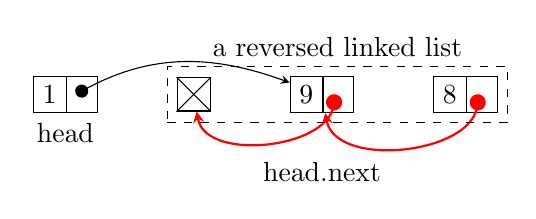
\begin{tikzpicture}[list/.style={rectangle split, rectangle split parts=2,
        draw, rectangle split horizontal}, >=stealth, start chain]
    
      \node[list,on chain] (A) {1};
      \node[on chain,draw,inner sep=6pt] (D) {};
      \draw (D.north east) -- (D.south west);
      \draw (D.north west) -- (D.south east);
      \node[list,on chain] (B) {9};
      \node[list,on chain] (C) {8};
    
      \draw[*->, red, thick] let \p1 = (C.two), \p2 = (C.center) in (\x1,\y2) to[out=-80,in=-80] (B);
      \draw[*->, red, thick] let \p1 = (B.two), \p2 = (B.center) in (\x1,\y2) to[out=-80,in=-80] (D);
      \draw[*->] let \p1 = (A.two), \p2 = (A.center) in (\x1,\y2) to[out=30,in=160] (B);
      \node[below=of A, yshift=1cm] (head){\alert{head}};
    
      \node[below=of B, yshift=.5cm] {\alert{head.next}};
    
      \node[fit=(B)(C)(D), dashed, draw](remain) {};
    
      \node[above=of remain, yshift=-1cm]{\alert{a reversed linked list}};
    \end{tikzpicture}
    
    \scalebox{.85}{  
        \begin{algorithm}[H]
            \caption{reverseList(head)}
            \If{head = null or head.next = null}{
                \Return{head}
            }
            $rest\gets reverseList(head.next)$ \\
            $head.next.next\gets head$ \\
            $head.next\gets null$\\
            \Return{rest}            
            \end{algorithm}
    }

\end{frame}

\begin{frame}
    \frametitle{2.4 Pros and Cons}
All recursions can be transformed into \textbf{iterative} algorithms. Generally, recursions make the code much cleaner, but they may result in several cons:

\begin{itemize}
    \item Slower.
    \item Larger memory overhead.
    \item Hard to analyze.
\end{itemize}

\end{frame}

\begin{frame}
\frametitle{Summary}

There are three important rules of thumb in developing recursive programs:

\begin{enumerate}
    \item The recursion has a \textbf{base case}.
    \item Recursive calls must address sub-problems that are \textbf{smaller} in some sense.
    \item Recursive calls should not address sub-problems that overlap.
\end{enumerate}
\end{frame}

\end{document}